\documentclass{article}

\usepackage{graphicx}
\usepackage{tikz}
\usepackage{tikzsymbols}
\usetikzlibrary{calc,patterns,shapes.geometric}
\pagestyle{empty}
\usepackage[margin=0pt]{geometry}
\geometry{papersize={14in,12in}}

\def\centerarc[#1](#2)(#3:#4:#5){\draw[#1] ($(#2)+({#5*cos(#3)},{#5*sin(#3)})$) arc (#3:#4:#5);}

\begin{document}
	\begin{figure}
		\centering
		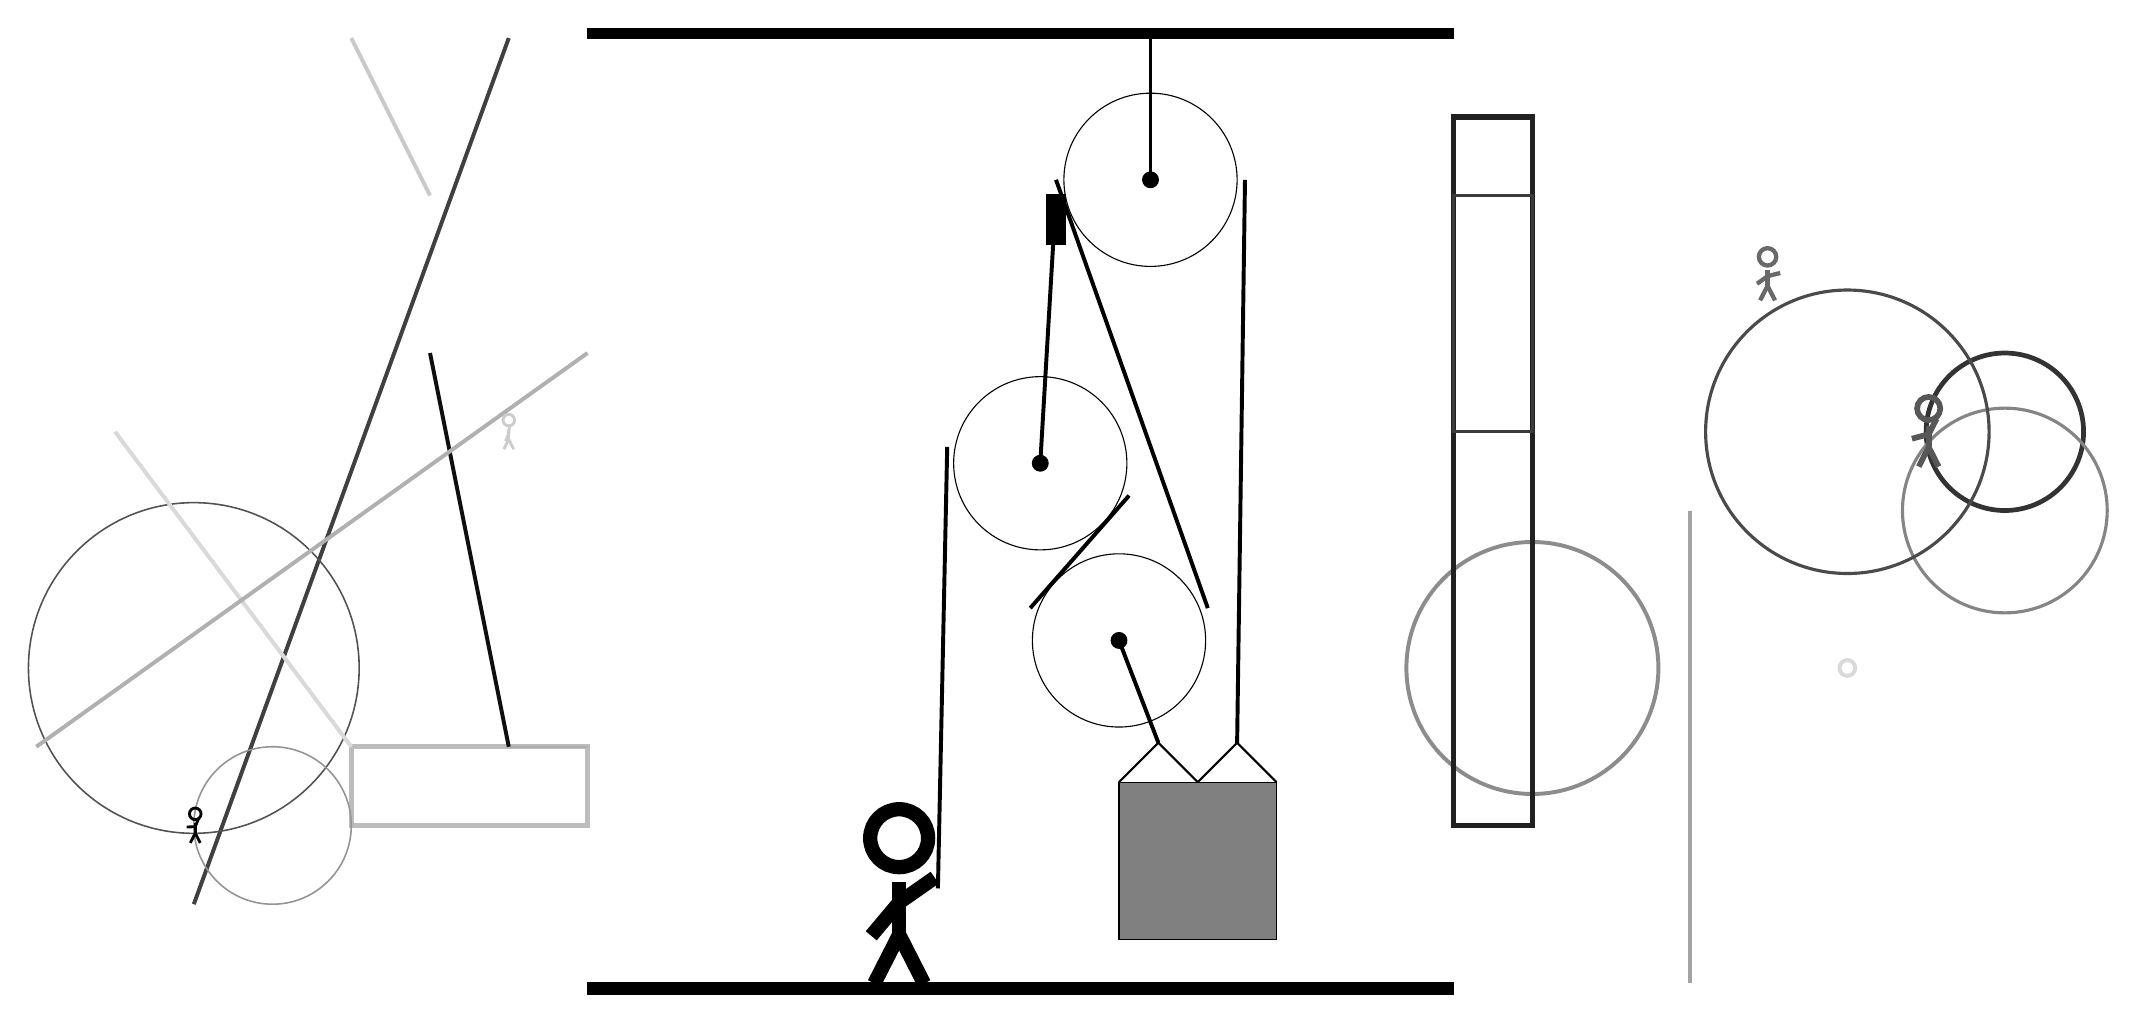
\begin{tikzpicture}
			%%%%% START %%%%%
			
			\draw[fill=black] (-6, 9) rectangle (5, 9.125);
			
			\draw[line width=0.7mm, color=black!26] (-6, -1) rectangle (-9, 0);
			
			\draw[line width=0.5mm, color=black!75](-7, 9) -- (-11, -2);
			\draw[line width=0.2mm, color=black!32] (-6, 0) rectangle (-7, 0);
			\draw [line width=0.2mm, color=black!68](-11, 1) circle (2.1);
			\draw [line width=0.5mm, color=black!45](6, 1) circle (1.6);
			\draw [line width=0.6mm, color=black!80](12, 4) circle (1.0);
			
			\draw [line width=0.4mm, color=black!48](12, 3) circle (1.3);
			\draw[line width=0.5mm, color=black!94](-7, 0) -- (-8, 5);
			\draw[line width=0.5mm, color=black!15](-9, 0) -- (-12, 4);
			
			\draw[line width=0.5mm, color=black!31](-6, 5) -- (-13, 0);
			\draw[line width=0.5mm, color=black!21](-9, 9) -- (-8, 7);
			\node[line width=0.5mm, color=black!59] at (9, 6) {\Strichmaxerl[3][36][14]};
			\draw[line width=0.4mm, color=black!72] (6, 2) rectangle (6, 0);
			
			\draw[line width=0.5mm, color=black!36](8, 3) -- (8, -3);
			\draw [line width=0.5mm, color=black!15](10, 1) circle (0.1);
			\node[line width=0.6mm, color=black!20] at (-7, 4) {\Strichmaxerl[2][69][83]};
			
			\node[line width=0.4mm, color=black!66] at (11, 4) {\Strichmaxerl[4][15][63]};
			
			\draw[line width=0.7mm, color=black!87] (5, -1) rectangle (6, 8);
			\draw [line width=0.2mm, color=black!42](-10, -1) circle (1.0);
			\node[line width=0.3mm, color=black!99] at (-11, -1) {\Strichmaxerl[2][2][68]};
			\draw[line width=0.4mm, color=black!77] (5, 7) rectangle (6, 4);
			
			\draw [line width=0.4mm, color=black!71](10, 4) circle (1.8);
			
			\draw (-0.25, 3.6) circle (1.1);
			\draw[fill=black] (-0.25, 3.6) circle (0.1);
			
			\draw (0.75, 1.35) circle (1.1);
			\draw[fill=black] (0.75, 1.35) circle (0.1);
			
			\draw (1.15, 7.2) circle (1.1);
			\draw[fill=black] (1.15, 7.2) circle (0.1);
			\draw[very thick] (1.15, 7.2) -- (1.15, 9);
			
			\draw[thick]  (0.75, -0.45) -- (1.25, 0.05) -- (1.75, -0.45) -- (2.25, 0.05) -- (2.75, -0.45);
			\draw[fill=black!50] (0.75, -0.45) rectangle (2.75, -2.45);
			
			\draw[line width=0.5mm] (-0.25, 3.6) -- (-0.05, 7.0);
			\draw[line width=0.5mm, fill=black](-0.15, 6.4) rectangle (0.05, 7.0);
			\draw[line width=0.5mm] (-1.55, -1.8) -- (-1.4318, 3.8083);
			\centerarc[line width=0.5mm](-0.25, 3.6)(-20:170:1.2000000000000002);
			\draw[line width=0.5mm] (0.8776, 3.1896) -- (-0.3776, 1.7604);
			\centerarc[line width=0.5mm](0.75, 1.35)(160:380:1.2000000000000002);
			\draw[line width=0.5mm] (1.8776, 1.7604) -- (-0.05, 7.2);
			\draw[line width=0.5mm](0.75, 1.35) -- (1.25, 0.05);
			\centerarc[line width=0.5mm](1.15, 7.2)(0:180:1.2000000000000002);
			\draw[line width=0.5mm] (2.35, 7.2) -- (2.25, 0.05);
			
			\node at (-2, -1.9) {\Strichmaxerl[10][50][35]};
			
			\draw[fill=black] (-6, -3) rectangle (5, -3.15);
			
			%%%%% END %%%%%
		\end{tikzpicture}
	\end{figure}	
\end{document}